\documentclass{article}
% Change "article" to "report" to get rid of page number on title page
\usepackage{amsmath,amsfonts,amsthm,amssymb}
\usepackage{setspace}
\usepackage{Tabbing}
\usepackage{fancyhdr}
\usepackage{lastpage}
\usepackage{extramarks}
\usepackage{chngpage}
\usepackage{soul,color}
\usepackage{graphicx,float,wrapfig}
\usepackage{multirow}
\usepackage{enumerate}
% In case you need to adjust margins:
\topmargin=-0.45in      %
\evensidemargin=0in     %
\oddsidemargin=0in      %
\textwidth=6.5in        %
\textheight=9.0in       %
\headsep=0.25in         %

% Homework Specific Information
\newcommand{\hmwkTitle}{Problem with "split-table"}
\newcommand{\hmwkClass}{}
\newcommand{\hmwkAuthorName}{Donglai\ Wei}


% Setup the header and footer
\pagestyle{fancy}                                                       %
\lhead{\hmwkAuthorName}                                                 %
\rhead{\firstxmark}                                                     %
\lfoot{\lastxmark}                                                      %
\cfoot{}                                                                %
\rfoot{Page\ \thepage\ of\ \pageref{LastPage}}                          %
\renewcommand\headrulewidth{0.4pt}                                      %
\renewcommand\footrulewidth{0.4pt}                                      %

% This is used to trace down (pin point) problems
% in latexing a document:
%\tracingall

%%%%%%%%%%%%%%%%%%%%%%%%%%%%%%%%%%%%%%%%%%%%%%%%%%%%%%%%\begin{enumerate}

% Some tools
\newcommand{\enterProblemHeader}[1]{\nobreak\extramarks{#1}{#1 continued on next page\ldots}\nobreak%
                                    \nobreak\extramarks{#1 (continued)}{#1 continued on next page\ldots}\nobreak}%
\newcommand{\exitProblemHeader}[1]{\nobreak\extramarks{#1 (continued)}{#1 continued on next page\ldots}\nobreak%
                                   \nobreak\extramarks{#1}{}\nobreak}%

\newlength{\labelLength}
\newcommand{\labelAnswer}[2]
  {\settowidth{\labelLength}{#1}%
   \addtolength{\labelLength}{0.25in}%
   \changetext{}{-\labelLength}{}{}{}%
   \noindent\fbox{\begin{minipage}[c]{\columnwidth}#2\end{minipage}}%
   \marginpar{\fbox{#1}}%

   % We put the blank space above in order to make sure this
   % \marginpar gets correctly placed.
   \changetext{}{+\labelLength}{}{}{}}%

\setcounter{secnumdepth}{0}
\newcommand{\homeworkProblemName}{}%
\newcounter{homeworkProblemCounter}%
\newenvironment{homeworkProblem}[1][Problem \arabic{homeworkProblemCounter}]%
  {\stepcounter{homeworkProblemCounter}%
   \renewcommand{\homeworkProblemName}{#1}%
   \section{\homeworkProblemName}%
   \enterProblemHeader{\homeworkProblemName}}%
  {\exitProblemHeader{\homeworkProblemName}}%

\newcommand{\problemAnswer}[1]
  {\noindent\fbox{\begin{minipage}[c]{\columnwidth}#1\end{minipage}}}%

\newcommand{\problemLAnswer}[1]
  {\labelAnswer{\homeworkProblemName}{#1}}

\newcommand{\homeworkSectionName}{}%
\newlength{\homeworkSectionLabelLength}{}%
\newenvironment{homeworkSection}[1]%
  {% We put this space here to make sure we're not connected to the above.
   % Otherwise the changetext can do funny things to the other margin

   \renewcommand{\homeworkSectionName}{#1}%
   \settowidth{\homeworkSectionLabelLength}{\homeworkSectionName}%
   \addtolength{\homeworkSectionLabelLength}{0.25in}%
   \changetext{}{-\homeworkSectionLabelLength}{}{}{}%
   \subsection{\homeworkSectionName}%
   \enterProblemHeader{\homeworkProblemName\ [\homeworkSectionName]}}%
  {\enterProblemHeader{\homeworkProblemName}%

   % We put the blank space above in order to make sure this margin
   % change doesn't happen too soon (otherwise \sectionAnswer's can
   % get ugly about their \marginpar placement.
   \changetext{}{+\homeworkSectionLabelLength}{}{}{}}%

\newcommand{\sectionAnswer}[1]
  {% We put this space here to make sure we're disconnected from the previous
   % passage

   \noindent\fbox{\begin{minipage}[c]{\columnwidth}#1\end{minipage}}%
   \enterProblemHeader{\homeworkProblemName}\exitProblemHeader{\homeworkProblemName}%
   \marginpar{\fbox{\homeworkSectionName}}%

   % We put the blank space above in order to make sure this
   % \marginpar gets correctly placed.
   }%

%%%%%%%%%%%%%%%%%%%%%%%%%%%%%%%%%%%%%%%%%%%%%%%%%%%%%%%%%%%%%



%%%%%%%%%%%%%%%%%%%%%%%%%%%%%%%%%%%%%%%%%%%%%%%%%%%%%%%%%%%%%
% Make title
\title{\vspace{0.3in}\textmd{\textbf{\hmwkTitle}}}
\date{2010.4.21}
\author{\textbf{\hmwkAuthorName}}
%%%%%%%%%%%%%%%%%%%%%%%%%%%%%%%%%%%%%%%%%%%%%%%%%%%%%%%%%%%%%

\begin{document}
\begin{spacing}{1.1}
\maketitle

\section{I)Corrected Pseudocode for split-table}

0) {\bf Settings:} \\ K nonempty dishes \\ Pick the Rth Restaurant with m tables.\\Pick the Tth($T\leq m$) tables with n($n\geq 2$) customers.\\ \\
1) {\bf 2-means++} 
\begin{enumerate}[(a)]
\item First 2 points:\\ \\
Randomly pick a customer C1 from table T to form a new table (m+1)\\
Randomly sample a dish(can be new) for the new table (m+1) according to the cost\\
Randomly sample another customer C2 from table t according to the cost\\
Randomly sample a dish(can be new) for the new table (m+2) according to the cost\\ \\
\item Initialization:\\ \\
For ww=randperm(customers from table T except C1,C2) \\ 
Randomly sample the table assignment zz$\in \{m+1,m+2\}$ for customer ww according to the cost\\
Randomly sample a dish(can be new) for table zz according to the cost\\
End \\ \\
\item Iteration(2-means):\\ \\
While no more changes of table config and dish config can increase P:\\
b=rand([0,1]) \\
Switch (ceil(b*4)):\\
case 1: Randomly pick a customer from table (m+1), assign it to table (m+2) if the change increase P\\
case 2: Randomly pick a customer from table (m+2), assign it to table (m+1) if the change increase P\\
case 3: pick table (m+1), assign it the dish which increase P mostly\\
case 4: pick table (m+2), assign it the dish which increase P mostly\\
End\\
\end{enumerate}  
\section{II)Controlled Experiment}
\subsection{a)Settings}
1) 40 Restaurants, each of which is a mixture of bars.\\
2) Erase table and dish config for the 1st Restaurant while keep the ground truth config for the rest.
\subsection{b)Goal}
Recover the table and dish config for the 1st Restaurant, conditioning on the rest.
\begin{figure}
    \centering 
    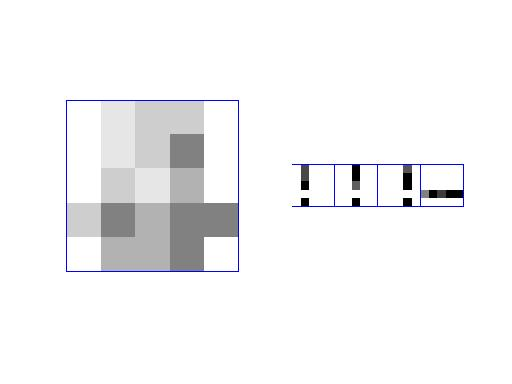
\includegraphics[width=3in,height=2in]{gt.jpg} 
    \caption{Table config for Restaurant 1 that gives lowest Free Energy}
\end{figure}

\subsection{c.1)Initialization--bottom up}
1) Initialization: In the 1st Restaurant, every customer has his own table and every table has its own dish.\\
2) Methods:\\
\begin{enumerate}
\item Local Search table(LS-t)+Local Search dish(LS-d):\\
The one in the middle is the Restaurant, around are table config results for different runs.\\
Clearly seen from below, though the local search works as well as fast, it can be hard to figure out the "row bar"
\begin{figure}[h] 
  \begin{minipage}[b]{0.5\textwidth} 
    \centering 
    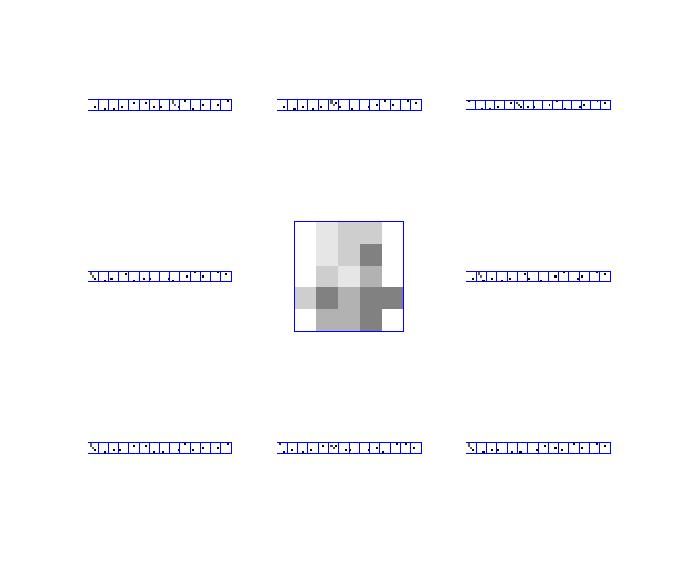
\includegraphics[width=3in,height=2in]{bu_lt.jpg} 
    \caption{LS-t once} 
    \label{fig:by:table} 
  \end{minipage}% 
  \begin{minipage}[b]{0.5\textwidth} 
    \centering 
    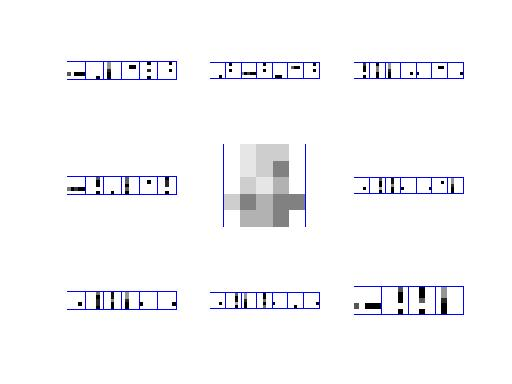
\includegraphics[width=3in,height=2in]{bu_lt_lk.jpg} 
    \caption{LS-t+LS-d+LS-t}
    \label{fig:by:table}  
   \end{minipage}% 
\end{figure}
\begin{figure}[h] 
  \begin{minipage}[b]{0.5\textwidth} 
    \centering 
    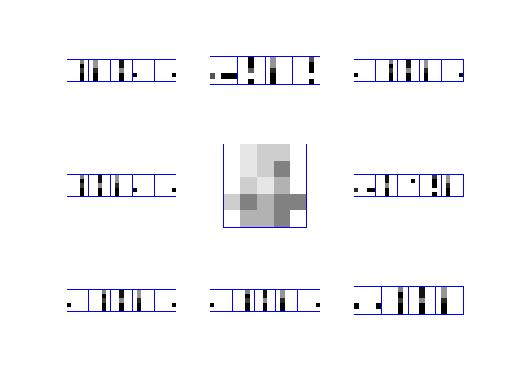
\includegraphics[width=3in,height=2in]{bu_lt_lk_lt.jpg} 
    \caption{LS-t+LS-d+LS-t+LS-d+LS-t}
    \label{fig:by:table} 
  \end{minipage}% 
  \begin{minipage}[b]{0.5\textwidth} 
    \centering 
    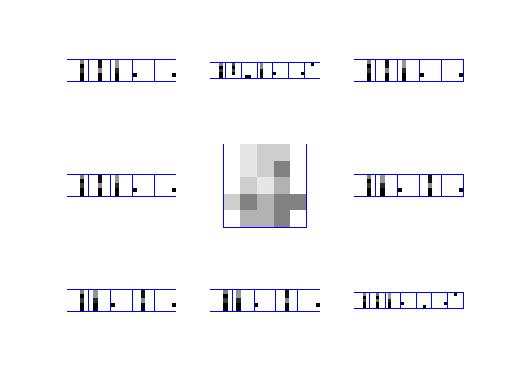
\includegraphics[width=3in,height=2in]{bu_lk.jpg} 
    \caption{LS-d+LS-t}
    \label{fig:by:table}  
   \end{minipage}% 
\end{figure}
\begin{figure}
    \centering 
    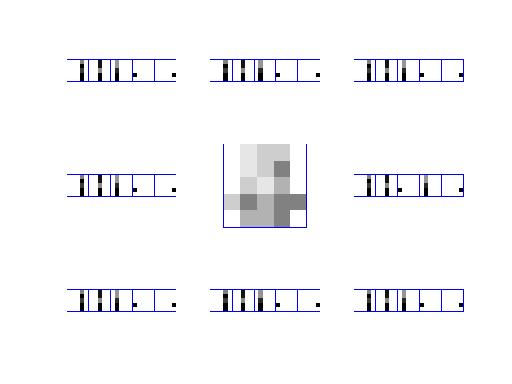
\includegraphics[width=3in,height=2in]{bu_lk_lt.jpg} 
    \caption{LS-d+LS-t+LS-d+LS-t}
\end{figure}



\item Merge table(M-t)+Merge dish(M-d):\\
\begin{figure}[h] 
  \begin{minipage}[b]{0.5\textwidth} 
    \centering 
    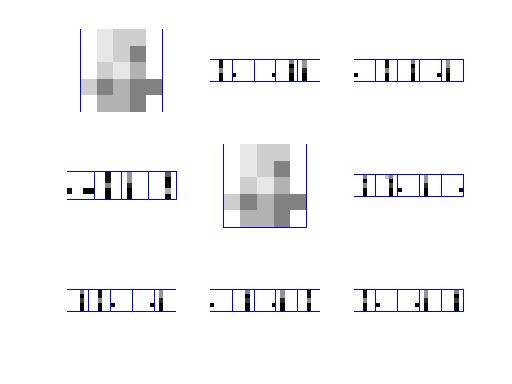
\includegraphics[width=3in,height=2in]{bu_mt.jpg} 
    \caption{Merge table once}
    \label{fig:by:table} 
  \end{minipage}% 
  \begin{minipage}[b]{0.5\textwidth} 
    \centering 
    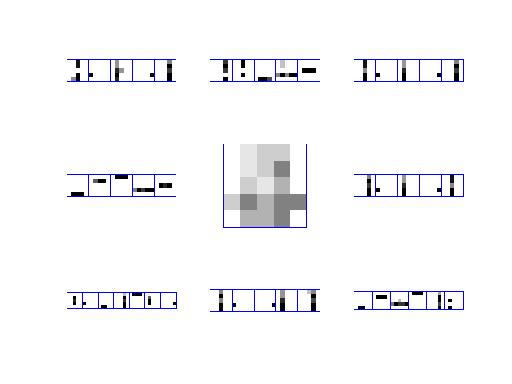
\includegraphics[width=3in,height=2in]{bu_md_mt.jpg} 
    \caption{Merge dish+Merge table}
    \label{fig:by:table}  
   \end{minipage}% 
\end{figure}

\item Comparisons of Random Combinations 
\begin{figure}[h] 
  \begin{minipage}[b]{0.5\textwidth} 
    \centering 
    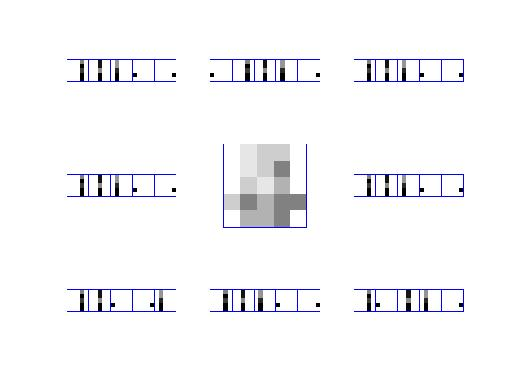
\includegraphics[width=3in,height=2in]{bu_l.jpg} 
    \caption{Random Combo of Local moves}
    \label{fig:by:table} 
  \end{minipage}% 
  \begin{minipage}[b]{0.5\textwidth} 
    \centering 
    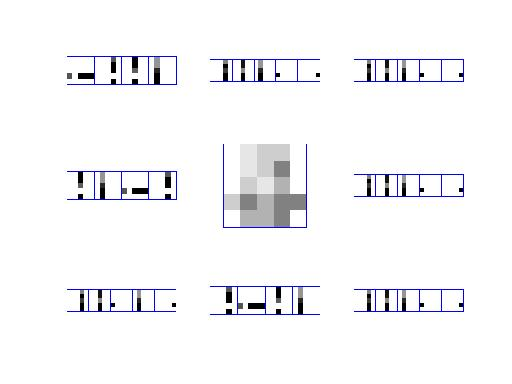
\includegraphics[width=3in,height=2in]{bu_m.jpg} 
    \caption{Random Combo of Merge moves}
    \label{fig:by:table}  
   \end{minipage}% 
\end{figure}
\begin{figure}[h] 
  \begin{minipage}[b]{0.5\textwidth} 
    \centering 
    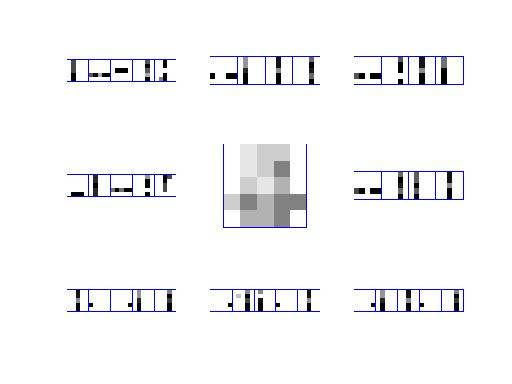
\includegraphics[width=3in,height=2in]{bu_ms.jpg} 
    \caption{Random Combo of Merge,Split moves}
    \label{fig:by:table} 
  \end{minipage}% 
  \begin{minipage}[b]{0.5\textwidth} 
    \centering 
    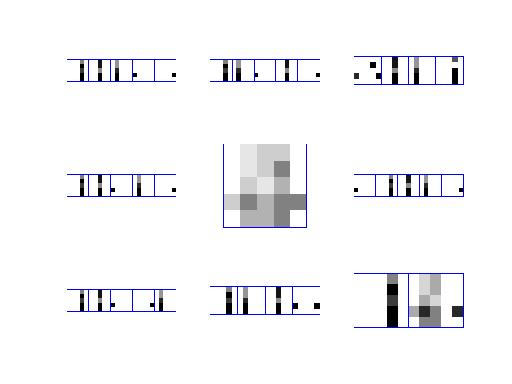
\includegraphics[width=3in,height=2in]{bu_lms.jpg} 
    \caption{Random Combo of Local,Merge,Split moves}
    \label{fig:by:table}  
   \end{minipage}% 
\end{figure}

\begin{figure}[h] 
  \begin{minipage}[b]{0.5\textwidth} 
    \centering 
    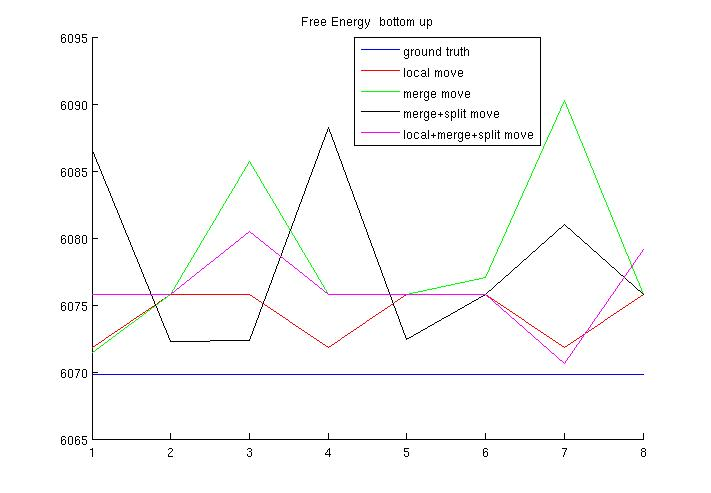
\includegraphics[width=3in,height=2in]{bu_energy2.jpg} 
    \caption{Free Energy corresponds to above config}
    \label{fig:by:table} 
  \end{minipage}% 
  \begin{minipage}[b]{0.5\textwidth} 
    \centering 
    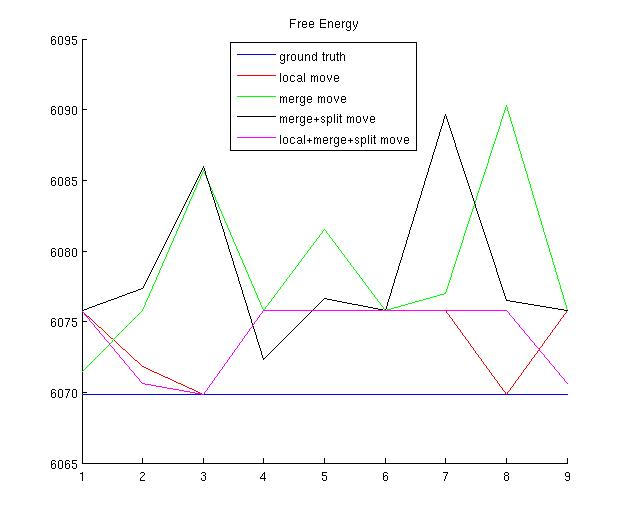
\includegraphics[width=3in,height=2in]{bu_energy.jpg} 
    \caption{Another run}
    \label{fig:by:table}  
   \end{minipage}% 
\end{figure}
\end{enumerate}

\subsection{c.1)Initialization--bottom up}
1) Initialization: In the 1st Restaurant, all customers have the same table which has a new dish.\\
2) Methods:\\
\begin{enumerate}
\item Local Search Move: As expected, the restaurant refuses to change.\\
\item Split Move:There is an "annealing" parameter$\alpha$(tuning weights) during sampling. So long $\alpha$ is not
too small or too big, the split moves give similar results. \\
\begin{figure}[h] 
  \begin{minipage}[b]{0.5\textwidth} 
    \centering 
    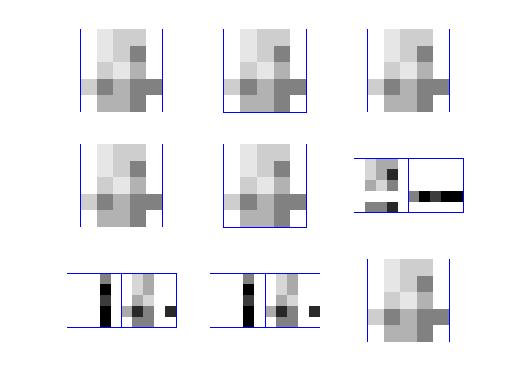
\includegraphics[width=3in,height=2in]{td_s_1.jpg} 
    \caption{Split table once}
    \label{fig:by:table} 
  \end{minipage}% 
  \begin{minipage}[b]{0.5\textwidth} 
    \centering 
    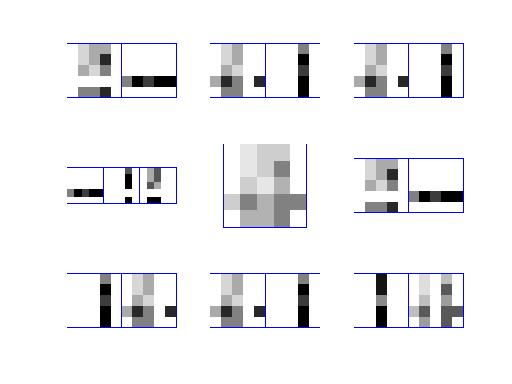
\includegraphics[width=3in,height=2in]{td_s_2.jpg} 
    \caption{Split table twice}
    \label{fig:by:table}  
   \end{minipage}% 
\end{figure}

\begin{figure}[h] 
  \begin{minipage}[b]{0.5\textwidth} 
    \centering 
    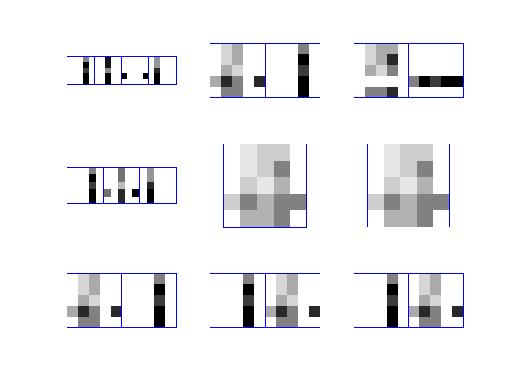
\includegraphics[width=3in,height=2in]{td_s_3.jpg} 
    \caption{Split table three times}
    \label{fig:by:table} 
  \end{minipage}% 
  \begin{minipage}[b]{0.5\textwidth} 
    \centering 
    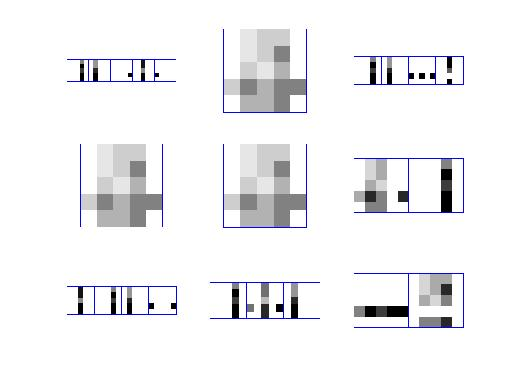
\includegraphics[width=3in,height=2in]{td_s_4.jpg} 
    \caption{Split table four times}
    \label{fig:by:table}  
   \end{minipage}% 
\end{figure}
\item Comparisons of Random Combinations 
\begin{figure}[h] 
  \begin{minipage}[b]{0.5\textwidth} 
    \centering 
    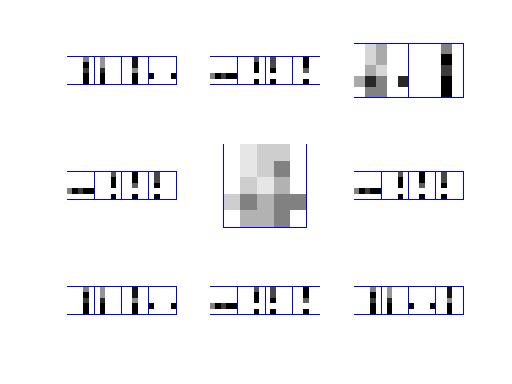
\includegraphics[width=3in,height=2in]{td_ms.jpg} 
    \caption{Random Combo of Merge,Split moves}
    \label{fig:by:table} 
  \end{minipage}% 
  \begin{minipage}[b]{0.5\textwidth} 
    \centering 
    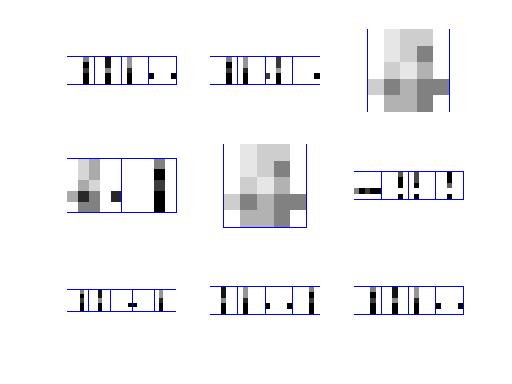
\includegraphics[width=3in,height=2in]{td_lms.jpg} 
    \caption{Random Combo of Local,Merge,Split moves}
    \label{fig:by:table}  
   \end{minipage}% 
\end{figure}

\begin{figure}[h] 
  \begin{minipage}[b]{0.5\textwidth} 
    \centering 
    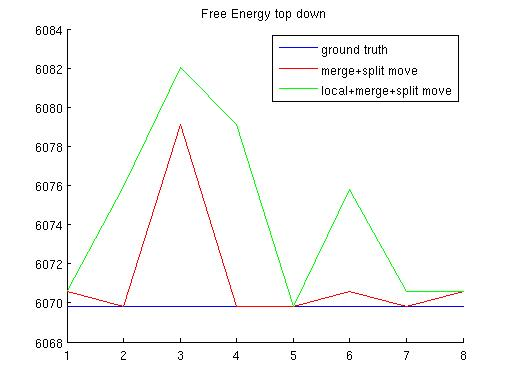
\includegraphics[width=3in,height=2in]{tf_energy.jpg} 
    \caption{Free Energy corresponds to above config}
    \label{fig:by:table} 
  \end{minipage}% 
  \begin{minipage}[b]{0.5\textwidth} 
    \centering 
    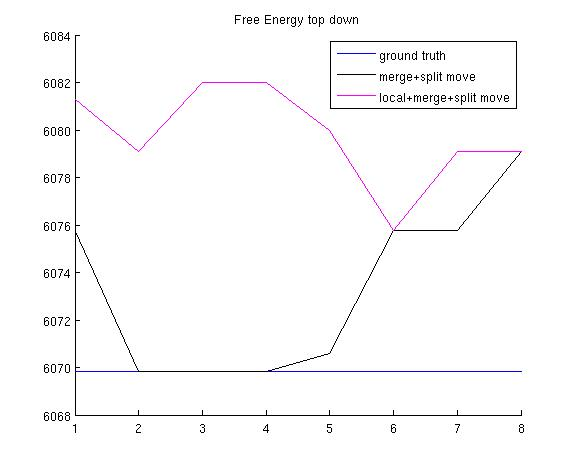
\includegraphics[width=3in,height=2in]{tf_energy2.jpg} 
    \caption{Another run}
    \label{fig:by:table}  
   \end{minipage}% 
\end{figure}
\end{enumerate}

\end{spacing}
\end{document}

%%%%%%%%%%%%%%%%%%%%%%%%%%%%%%%%%%%%%%%%%%%%%%%%%%%%%%%%%%%%%
